\documentclass[11pt, oneside]{article}   	% use "amsart" instead of "article" for AMSLaTeX format
\usepackage{geometry}                		% See geometry.pdf to learn the layout options. There are lots.
\geometry{letterpaper}                   	% ... or a4paper or a5paper or ... 
%\geometry{landscape}                		% Activate for rotated page geometry
\usepackage[parfill]{parskip}    	% Activate to begin paragraphs with an empty line rather than an indent
\usepackage{graphicx}				% Use pdf, png, jpg, or eps§ with pdflatex; use eps in DVI mode
								% TeX will automatically convert eps --> pdf in pdflatex		
\usepackage{amssymb}
\usepackage{amsmath}
\usepackage{enumitem}
\usepackage{hyperref}
\hypersetup{
    colorlinks=false,
    linkcolor=blue,
    filecolor=magenta,      
    urlcolor=cyan,
    pdftitle={Overleaf Example},
    pdfpagemode=FullScreen,
    }

%SetFonts

%SetFonts


\title{Predicting Global Agricultural Crop Yield}
\author{Sungjoon Park}
\date{February 16, 2024}		% Activate to display a given date or no date

\begin{document}
\maketitle
\begin{abstract}
This research proposes a deep neural network model that predicts global agricultural supply by analyzing global climate images, aiming to address the inefficiencies of current region-specific models. Utilizing a combination of CNNs and LSTM networks, the model processes climate imagery to extract features for accurate global crop yield predictions. The model’s performance will be benchmarked against traditional prediction models using the mean squared error (MSE) metric to ensure its effectiveness and applicability.
\end{abstract}

\section*{Introduction}

Since the advent of the 2010s, the volatility in the supply of agricultural products has seen a significant increase, largely attributed to the effects of global warming. This has led to a widening imbalance between supply and demand, culminating in a surge in the prices of agricultural products, a phenomenon known as ‘agflation’. The ripple effect of this surge poses a risk of triggering global inflation. Consequently, the urgency and importance of accurately predicting global agricultural supply in a timely manner have been brought to the forefront.

Existing models for predicting crop yields, however, are predominantly region-specific \cite{citation_key1}\cite{citation_key3}. While these models exhibit commendable performance in predicting crop yields within their respective regions, they often exhibit heterogeneity across different regions. The features input into the model or the machine learning algorithms employed may vary significantly. As such, the utilization of these individual models for global crop yield prediction can result in substantial time and cost implications for data collection and analysis. This underscores the need for a more efficient and globally applicable model for predicting crop yields.

In response to this challenge, this research proposes a novel approach: the use of a deep neural network trained to predict global agricultural product supply using global climate information as input. This approach necessitates the incorporation of not only traditional structured data but also unstructured data such as images. Image data, such as global average temperature maps, effectively characterize and summarize the current status of global climate, providing valuable input for our model. The performance of this model will be evaluated against representative prediction models in economic literature, using the mean squared error (MSE) as the metric.

\section*{Related Work}

Klumpenburg et al. (2020) \cite{citation_key3} conducted a comprehensive review of the existing literature to identify the major research questions pertaining to crop yield prediction. These questions can be distilled into three primary inquiries: Which machine learning algorithms have been employed in the literature for crop yield prediction? What features have been utilized in the literature for crop yield prediction using machine learning? And what evaluation parameters and approaches have been adopted in the literature for crop yield prediction?

In response to the first research question, Klumpenburg et al. enumerated 37 features that have been used in the reviewed papers. Among these, seven features—temperature, soil type, rainfall, crop information, soil maps, humidity, and pH-value—account for 50\% of the usage. The study also highlighted the most frequently used machine learning algorithms: neural networks, linear regression, random forest, support vector machine, and gradient boosting tree. Neural networks were used 27 times, constituting 40.2\% of the total cases, thereby indicating their recognition as the most accurate predictor by researchers. However, it is important to note that these neural networks were specifically used for predicting regional crop yield, not for global prediction.

Lastly, the study found that previous research primarily used evaluation parameters derived from the mean square error (MSE), namely the root mean square error (RMSE), R-squared, and MSE. These methods accounted for 73.6\% of the total cases. In other instances, researchers employed the mean absolute error (MAE), which is robust to outliers, the mean absolute percentage error (MAPE), and the reduced simple average ensemble (RSAE), among others.

\section*{Proposed Work}

This research project utilizes images as input data and generates numerical values as output. The proposed neural network architecture commences with Convolutional Neural Networks (CNN), which process the images to produce encoded latent representations. Subsequently, these representations are input sequentially into a Long Short-Term Memory (LSTM) network. The culmination of this process is the LSTM network synthesizing the inputs from multiple CNNs to output a singular predictive value for global crop yield.

To elucidate, the architecture employs several CNNs that process global climate imagery to extract pertinent features. These features are then conveyed to the LSTM network, which functions within a many-to-one feed-forward process, enabling the generation of a consolidated prediction.

The development of this network will involve modifications to the existing model, informed by prior research that integrates CNNs with Recurrent Neural Networks (RNN), or the construction of a predictive model via fine-tuning. Notably, while the application domains differ, relevant studies, such as that by Gheisari et al. (2021) \cite{citation_key2}, provide a foundation. Their research delineates a model for glaucoma detection—predominantly responsible for blindness—wherein spatial features derived from CNNs are fed into each RNN layer, and temporal features are subsequently outputted. Given the architectural similarities, it is plausible to base our model on these antecedent frameworks.

Furthermore, the project aims to address the challenge of incorporating global common features that influence crop yield into the CNN-LSTM structure. One potential approach involves introducing these features at the LSTM layers, alongside the CNN outputs. Alternatively, the integration of an ancillary fully-connected layer preceding the LSTM’s output layer may serve to encapsulate these features. The selection of the optimal method will be predicated on its contribution to enhancing predictive accuracy.

\section*{Datasets}

\begin{enumerate}
\item \textbf{Input data (Climate Information)}
	\begin{enumerate}[label=(\alph*)]
	\item \textbf{Near-Surface Air Temperature Monthly Data} \\
	- Source: \href{https://cds.climate.copernicus.eu/}{C3S} (Copernicus Climate Change Service) \\
	- Period: Jan. 2015 $\sim$ \\
	\begin{figure}[htbp]
    		\centering
	    \begin{minipage}{0.6\textwidth}
    		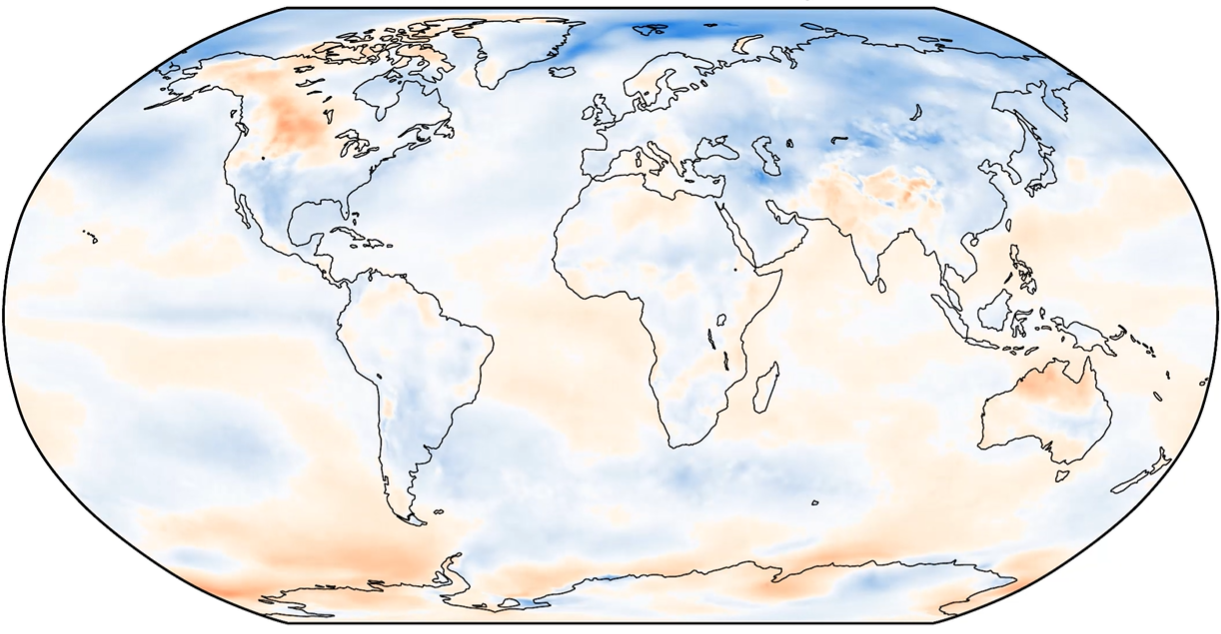
\includegraphics[width=\textwidth]{images/image_for_proposal_1.png}
	    \end{minipage}%%%

    		\begin{minipage}[t]{0.6\textwidth}
	    \caption{Near-Surface Air Temperature sample}
    		\label{fig1}
   	 	\end{minipage}%%%
	\end{figure}
	\item \textbf{Global Monthly Precipitation} \\
	- Source: \href{https://cds.climate.copernicus.eu/}{C3S} (Copernicus Climate Change Service) \\
	- Period: Jan. 1979 $\sim$ Dec. 2022 \\
	\begin{figure}[htbp]
    		\centering
	    \begin{minipage}{0.6\textwidth}
    		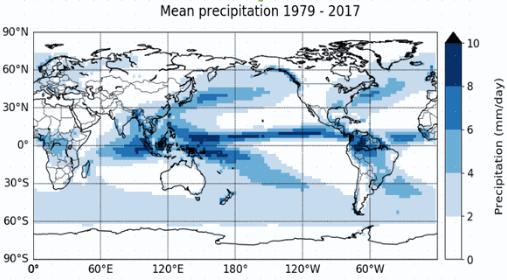
\includegraphics[width=\textwidth]{images/image_for_proposal_2.png}
	    \end{minipage}%%%

    		\begin{minipage}[t]{0.6\textwidth}
	    \caption{Global Precipitation sample}
    		\label{fig1}
   	 	\end{minipage}%%%
	\end{figure}
	\end{enumerate}
\item \textbf{Output data (Crop Yield)} \\
- Source: \href{https://ourworldindata.org/crop-yields#explore-data-on-crop-yields}{Our World in Data} \\
- Period: 1275 $\sim$ 2021 \\
- Types: Wheat, Rice, Soybean, etc.
\end{enumerate}

\section*{Evaluation - To be completed}

The principal objective of this research is to address a regression problem, wherein the output layer of the neural network is meticulously engineered to predict crop yield with high precision. Consequently, the primary metric for evaluation will be mean square error (MSE) or its derivatives, such as root mean square error (RMSE) or the coefficient of determination, commonly referred to as R-squared.

\section*{Timeline}

\begin{enumerate}
\item \textbf{Phase 1}: 2/16 $\sim$ 2/20
	\begin{enumerate}[label=(\alph*)]
	\item Before getting into modeling phases, other features that can potentially affect crop yield will be added to supplement global climate information. I look into them by reviewing a survey paper on crop yield prediction \cite{citation_key3}.
	\item While necessary features being selected in the first module, the model architecture that can incorporate a convolutional neural network into a many-to-one ecurrent neural network will be selected.
	\end{enumerate}

\item \textbf{Phase 2}: 2/21 $\sim$ 3/10 \\
In this phase, three separate modules will be implemented. The outperforming module will be chosen as the final neural network model.
	\begin{enumerate}[label=(\alph*)]
	\item \textbf{Module 1} \\
	In this module, I attempt to increase the number of data to train a deep neural network by applying methods such as cropping.
	\item \textbf{Module 2} \\
	In this module, I apply self-supervised learning methodologies to train a deep neural network with insufficient number of samples.
	\item \textbf{Module 3} \\
	I search for a pre-trained model to fine-tune for the purpose of this project.
	\end{enumerate}

\item \textbf{Phase 3}: 3/11 $\sim$ 3/29 \\
I compare the prediction performance of the selected model in the Phase 2 to the popular model in economic literature. Moreover, I conduct hyperparameter-tuning to enhance the neural network's performance.

\item \textbf{Phase 5}: 3/30 $\sim$ 4/20 \\
I reflect feedback on the interim results, and improve the model performance.

\item \textbf{Phase 6}: 4/21 $\sim$ 4/30 \\
I Compose final deliverables: video, final report and presentation.
\end{enumerate}

\section*{Conclusion}

This study explores the potential of combining CNN and LSTM network in predicting crop yields by utilizing temperature and precipitation maps. This approach allows for the integration of climate data into predictive models. Furthermore, the model is designed to simultaneously predict global crop yields using information from around the world. Given the significant impact of agricultural products on inflation, a phenomenon recently termed as ‘agflation’, and the increasing variability in agricultural supply across different regions due to climate changes, the accurate and timely prediction of global agricultural product prices becomes crucial. In the context of global warming, this model serves as a valuable tool for economists, enabling them to effectively predict and respond to changes in the global agricultural market.

\begin{thebibliography}{9}

\bibitem{citation_key1}
Ansarifar, J., Wang, L., \& Archontoulis, S. V. (2021). An interaction regression model for crop yield prediction. \textit{Scientific reports}, 11(1), 17754. https://doi.org/10.1038/s41598-021-97221-7

\bibitem{citation_key2}
Gheisari, S., Shariflou, S., Phu, J., Kennedy, P. J., Agar, A., Kalloniatis, M., \& Golzan, S. M. (2021). A combined convolutional and recurrent neural network for enhanced glaucoma detection. \textit{Scientific Reports 11, 1945.} https://doi.org/10.1038/s41598-021-81554-4

\bibitem{citation_key3}
Klompenburg, T.V., Kassahun, A., \& Catal, C. (2020). Crop yield prediction using machine learning: A systematic literature review. \textit{Comput. Electron. Agric., 177}, 105709.

\end{thebibliography}

\end{document} 